\documentclass[14pt]{extarticle}

\usepackage[utf8]{inputenc}
\usepackage[english]{babel}
\usepackage[T2A]{fontenc}
\usepackage{url}
\usepackage{booktabs}
\usepackage{amsfonts}
\usepackage{nicefrac}
\usepackage{microtype}
\usepackage{amsthm}
\usepackage{multirow}
\usepackage{bm}
\usepackage{mathrsfs}
\usepackage{lipsum}
\usepackage{graphicx}
\usepackage{natbib}
\usepackage{wrapfig}
\usepackage{doi}
\newtheorem{theorem}{Theorem}[section]
\newtheorem{corollary}{Corollary}[theorem]
\renewcommand{\abstractname}{Аннотация}

\usepackage{mathtools}
\usepackage{amsmath}
\DeclareMathOperator*{\argmax}{arg\,max}
\DeclareMathOperator*{\argmin}{arg\,min}
\usepackage[dvipsnames]{xcolor}

\title{Predictive multitask model selection using symbolic regression methods}
% Выбор предсказательной модели в режиме многозадачного обучения с применением методов символьной регрессии.

\author{
    Muhammadsharif Nabiev \\
    Department of Intelligent Systems\\
    MIPT\\
    \texttt{nabiev.mf@phystech.edu} \\
    % \And
    % Oleg Bakhteev \\
    % Department of Intelligent Systems\\
    % MIPT\\
    \texttt{} \\
}
\date{}

% \renewcommand{\shorttitle}{Inductive bias in model selection}

\hypersetup{
pdftitle={Inductive bias in model selection},
pdfsubject={q-bio.NC, q-bio.QM},
pdfauthor={Muhammadsharif},
pdfkeywords={model selection, evolutionary algorithm},
}

\begin{document}
% \maketitle

\thispagestyle{empty}

\begin{titlepage}
    \begin{center}
        \textsc{Московский физико-технический институт}\\
        (национальный исследовательский университет)\\
        \textsc{Физтех-школа прикладной математики и информатики}\\
        \textsc{Кафедра интеллектуальных систем}
    \end{center}
    \vspace{2.5cm}
    \begin{center}
        {Набиев Мухаммадшариф Фуркатович}
        \par
        \vspace{2cm}
        {\Large \textsc{\textbf{Выбор предсказательной модели в режиме многозадачного обучения с применением методов символьной регрессии}}}
        \par
        % \vspace{2cm}
        % {03.04.01~--- Прикладные математика и физика}
        \par
        \vspace{2cm}
        \textsc{Выпускная квалификационная работа бакалавра}
    \end{center}
    \vspace{2cm}
    \hfill\parbox{8,4cm}{\textbf{Научный руководитель:}
    \\к.ф.-м.н. О.\,Ю.\,Бахтеев}
    \par
    \vspace{1.5cm}
    \begin{center}
        {Москва~--- 2025}
    \end{center}
\end{titlepage}
\setcounter{page}{2}
%------------------------------------------------------------------------------------------------------------
\newpage
\begin{center}
    \Large{\textbf{Abstract}}
\end{center}
This paper tackles the problem of constructing suboptimal models within multitask learning paradigm. Given a set of intrinsically related tasks, the goal is to uncover a shared structure—known as the inductive bias—across all tasks. By applying constrained evolutionary symbolic regression, we show that these models can be decomposed in a way that reveals the tasks' underlying structure. We conduct experiments on synthetic data and dataset of numbers MNIST, where the data structure, generation process, and optimal models are known. The results indicate that the models produced by the proposed method are indeed optimal for their respective tasks.
%------------------------------------------------------------------------------------------------------------
\newpage
\tableofcontents
%------------------------------------------------------------------------------------------------------------
\newpage
\section{Introduction} 
The problem of establishing inductive bias~\citep{Mitchell2007TheNF} is a fundamental in  machine learning. Inductive bias encapsulates the core assumptions that underpin the methodology adopted by a particular model in its predictive endeavors. For example, convolution captures locality of data and recurrent neural networks take into account sequential dependency~\citep{cohen2017inductivebiasdeepconvolutional, DUBININ2024106179}. It extends beyond the boundaries of explicitly observed data. Understanding and leveraging inductive bias is essential for enhancing model performance, especially in complex environments where data may exhibit diverse characteristics. 


Inductive bias refers to a model's set of assumptions that guide it in making predictions on unseen data. These assumptions are essential for generalization: without them, a model would treat every possible hypothesis as equally likely, leading to overfitting or poor predictive performance~\citep{Mitchell2007TheNF}. Different datasets often possess unique distinguishing features that can be exploited for improved performance. For instance, models trained on image data may benefit from biases related to spatial hierarchies~\citep{alex_net}, while those handling sequential data~\citep{lstm, Vaswani2017AttentionIA}, such as time series or text, may rely on temporal dependencies. Recognizing and systematically integrating these biases into the model selection process can facilitate the identification of suboptimal yet effective architectures.

However, incorporating inductive biases into automated model selection remains a non-trivial challenge. In recent years, the field of machine learning has experienced rapid advancements driven by the development of sophisticated algorithms and architectures capable of tackling a wide range of tasks~\citep{SHEHAB2022105458, OZBAYOGLU2020106384, ml_in_cv_survey, 10803211}, from natural language processing~\citep{brown2020languagemodelsfewshotlearners} to computer vision~\citep{NIPS2012_c399862d}. However, the design and optimization of these models often require significant expertise and resources, leading to the rise of automated machine learning (AutoML) systems~\citep{He_2021}. These systems are designed to simplify the process of choosing and tuning models, making machine learning tools more accessible and easier to use.

We use symbolic regression to infer inductive bias. Symbolic regression methods belong to a broader class of approaches that reduce the need for extensive manual tuning of model architectures. These methods aim to automatically discover symbolic representations using search strategies such as evolutionary algorithms~\citep{cosmo_ind_bias_sym_regression}. 
Few notable approaches are AutoML-Zero\citep{automl-zero} and PySR~\citep{Cranmer2023InterpretableML}, which autonomously construct models using a genetic programming framework, assembling them from fundamental mathematical operations. These methods represent a significant departure from traditional model selection paradigms, which typically rely on predefined structures~\citep{alex_net} or human intuition~\citep{zoph2016neural}. By allowing the model architecture to emerge organically from the data, AutoML-Zero and PySR minimizes biases introduced by prior knowledge, potentially leading to the discovery of novel architectures better suited to the task at hand~\citep{Dorrell2022MetaLearningTI, Liu2024KANKN}.


By applying symbolic regression within a multitask learning framework, we aim to uncover shared inductive biases. Multitask learning (MTL) is closely linked to the notion of inductive bias. In fact, multitask learning can be viewed as a mechanism for introducing a meta-level inductive bias~\citep{multitask_ind_bias, baxter_ind_bias}---one that promotes the learning of shared representations across multiple related tasks. By jointly training on several tasks, the model is encouraged to capture common structures or features that are beneficial across them, effectively embedding a bias that reflects inter-task regularities. This shared inductive bias can improve generalization, especially when individual tasks have limited data or when the tasks exhibit complementary structure. Thus, multitask learning not only enhances performance through knowledge transfer but also serves as a principled way to shape the hypothesis space in alignment with the underlying relationships among tasks~\citep{survey_mtl}. 


While MTL and symbolic regression can discover models with shared representations, these often risk encoding irrelevant features. To address this, the Information Bottleneck (IB) principle~\citep{Tishby2000TheIB} provides a framework for learning compressed, task-relevant representations by maximizing mutual information with outputs while minimizing it with inputs. In deep learning, is has applications such as explanation of how neural nets learn~\citep{ShwartzZiv2017OpeningTB}, and methods such as Variational Information Bottleneck~\citep{Alemi2017DeepVI}. There were also attempts to combine IB with MTL~\citep{Qian2020MultiTaskVI}.

In this paper, we investigate how inductive biases inherent in the data can guide model selection within the multitask learning framework. We propose an automated methodology that combines evolutionary algorithms with symbolic regression to explore a diverse range of shared model architectures. A single model is trained with multiple task-specific heads corresponding to different datasets, enabling the discovery of shared representations that capture common structures across tasks. To ensure these representations remain compact and focused on relevant information, we incorporate the Information Bottleneck principle, which encourages learning compressed, task-relevant features, see fig.~\ref{3d-paretto-front}. This approach aims to improve generalizations and adaptability while reducing the need for extensive manual tuning by systematically searching for architectures that balance shared and task-specific components effectively. 

Our contributions include:
\begin{enumerate}
    \item We propose model selection criterion to identify inductive bias for a given set of tasks.
    \item We provide theoretical justifications for the proposed method.
    \item The experiments demonstrate that models achieving optimal trade-offs between accuracy, information, and complexity lie on the Pareto front.
\end{enumerate}

\begin{figure}[hbt!]
    \centering
    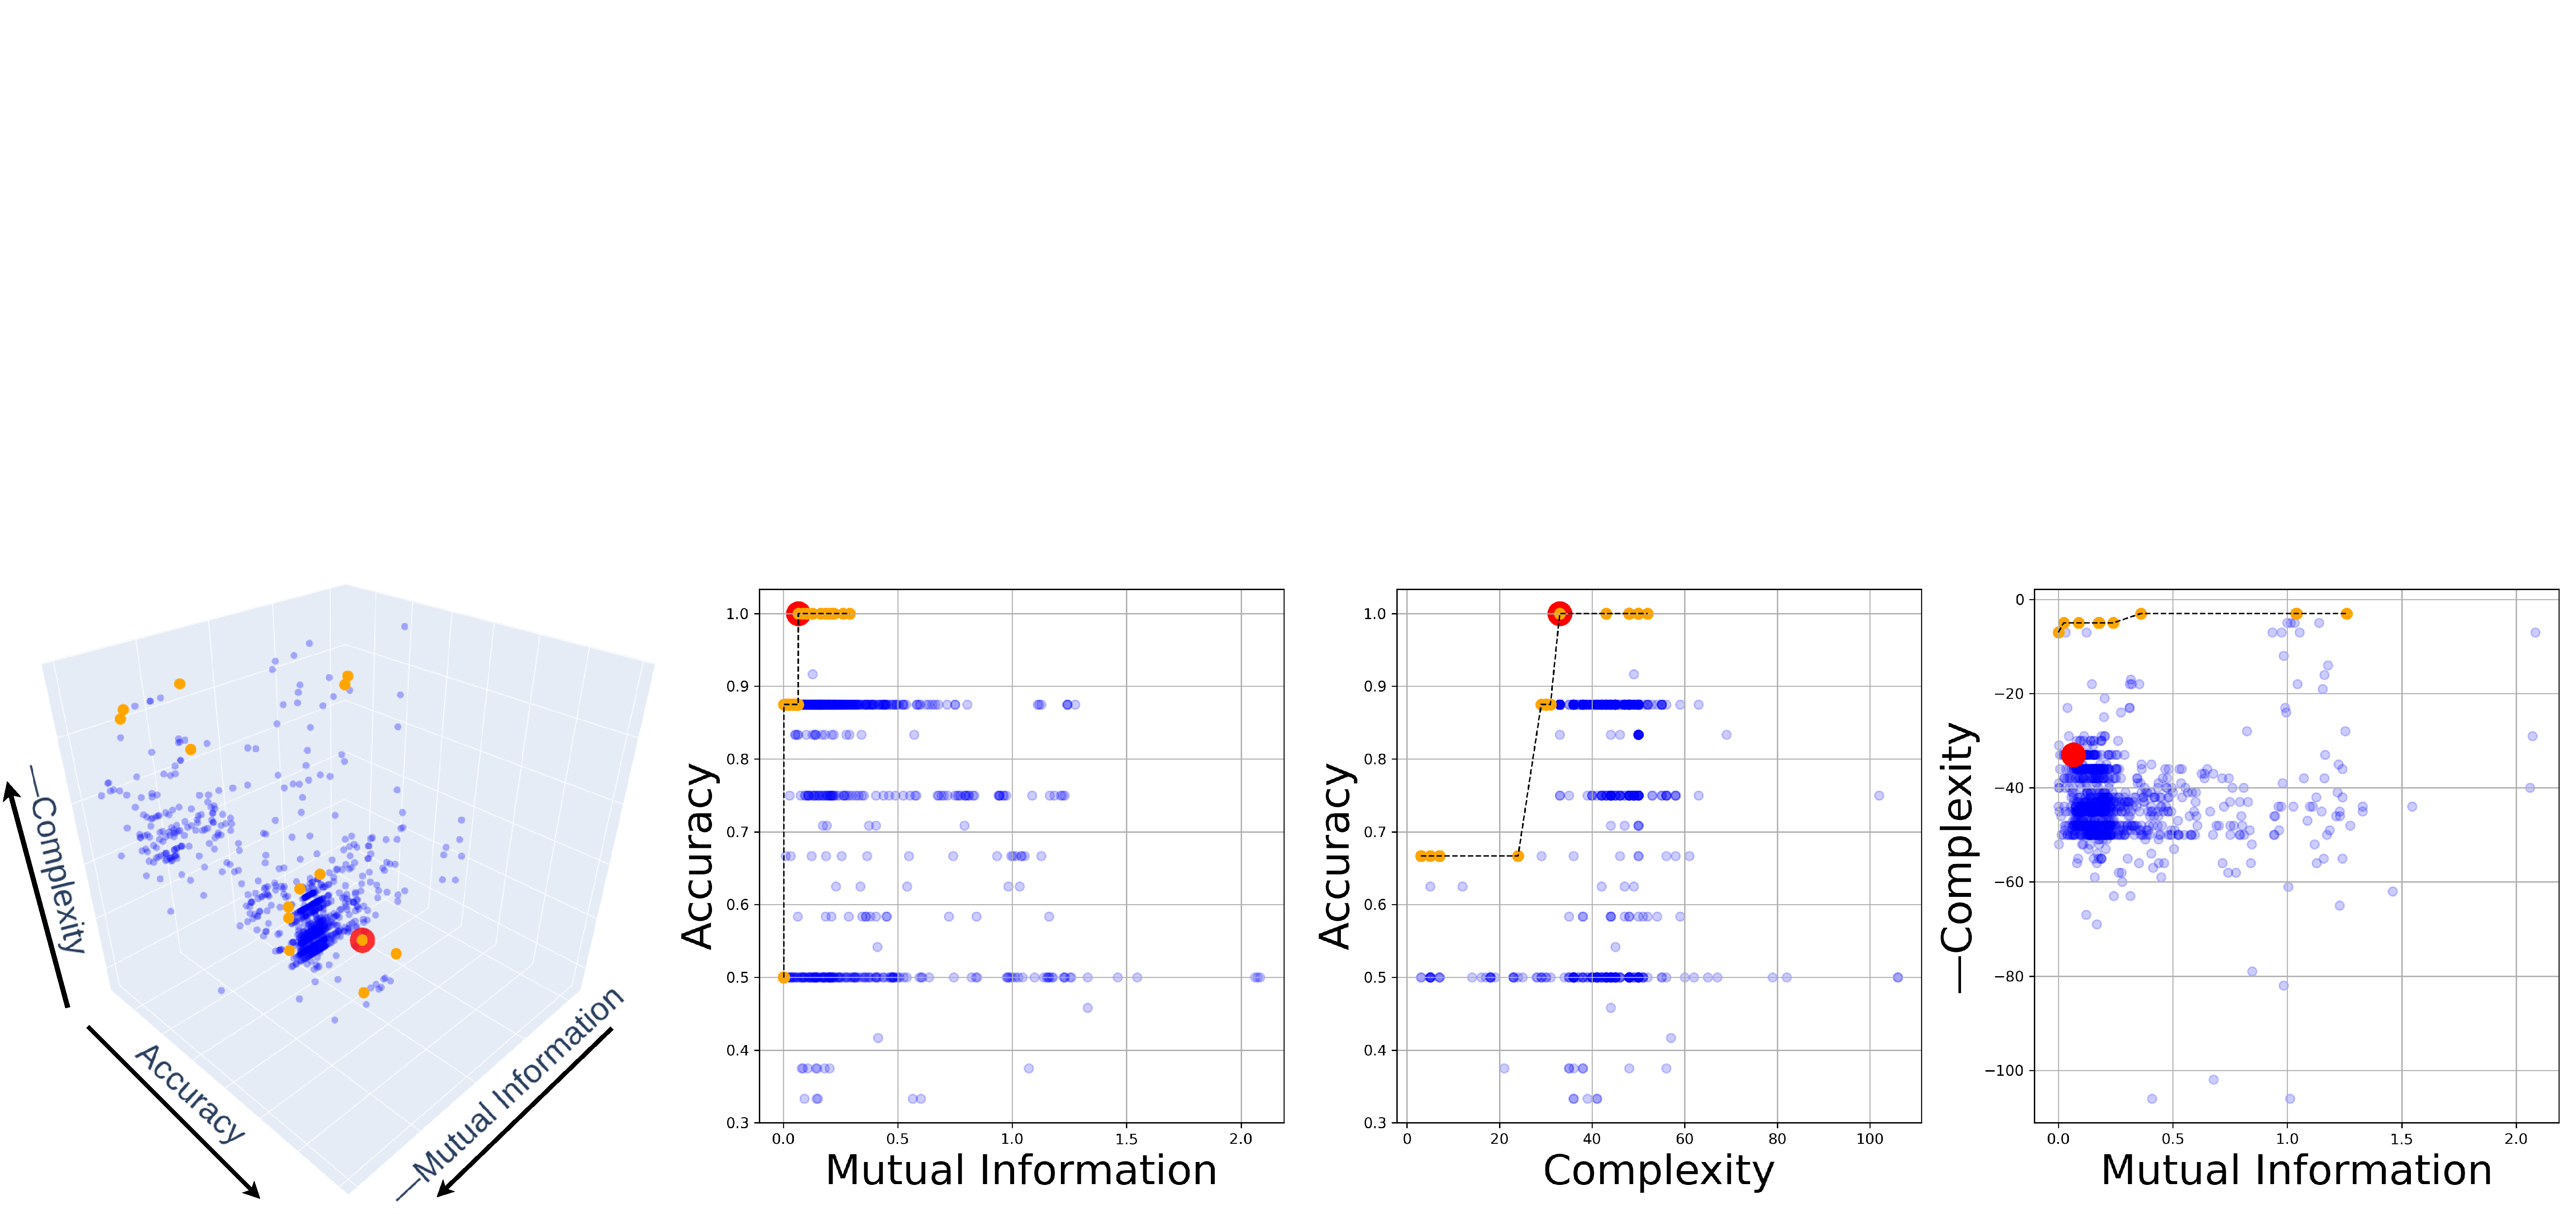
\includegraphics[width=1\textwidth]{3d_paretto.drawio.pdf}
    \caption{3D and 2D scatter plots illustrate the performance of discovered models across three objectives: Mutual Information, Accuracy and Complexity. Each blue point corresponds to a candidate model, while the red point denotes the ground-truth model. The ground-truth model lies on Pareto-front for the Accuracy-Mutual Information and Accuracy-Complexity projections, indicating its optimality with respect to these trade-offs. In the Complexity-Mutual Information plane, the presence of models that are both low-complexity and low-information is expected, as such models represent simple expressions and ignore the input.}
    \label{3d-paretto-front}
\end{figure}
%------------------------------------------------------------------------------------------------------------
\newpage
\section{Problem statement}
    Multitask setting is based on an assumption that tasks can serve as mutual sources of inductive bias~\citep{multitask_ind_bias}. Let \( \mathfrak{T} = \{T_1, T_2, \dots, T_m\} \) be a set of tasks. These tasks share a common internal structure but differ in their output heads, see fig.~\ref{expression_tree}. Each task \( T_i \) has its corresponding dataset \( \mathfrak{D}_i = (\mathbf{X}^i, \mathbf{y}^i) \) with an input objects \(\mathbf{X}^i \in \mathbb{R}^{N_i \times n}\) and output targets \(\mathbf{y}^i \in \mathcal{Y}\) where \(\mathcal{Y}=\mathbb{R}^{N_i}\) for regression and \(\mathcal{Y} = \{1, \dots, K\}^{N_i}\) for classification. 

    \begin{figure}[hbt!]
    \centering
    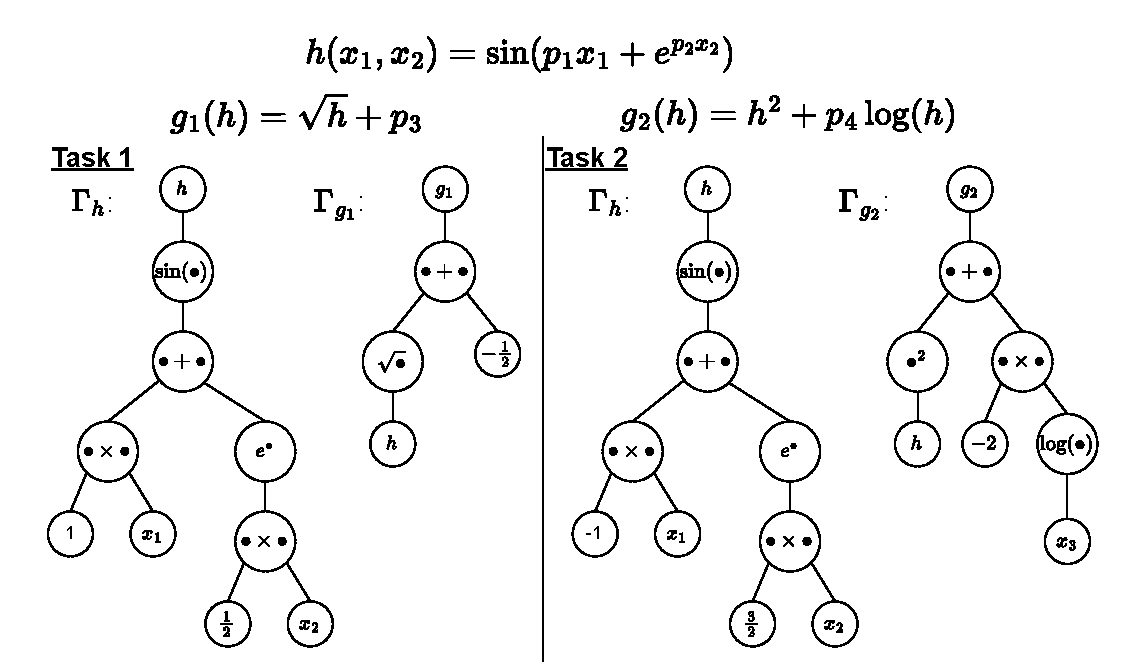
\includegraphics[width=1\textwidth]{expression_tree.drawio.pdf}
    \caption{Multitask setting for \(m=2\) tasks. Dimension of hidden space \(d=1\). Parameters are task-specific and correspond to tasks.}
    \label{expression_tree}
    \end{figure}

    A \textit{model} \(\mathbf{f}(\mathbf{x}, \mathbf{w})\) is defined as an expression with the following mapping \(\mathbb{R}^n \times \mathbb{R}^l \rightarrow \mathbb{R}^m\), whose \textit{structure} \(\Gamma_\mathbf{f} \in \mathfrak{G}\) can be represented via expression tree~\citep{RudStr13, KULUNCHAKOV2017221} and \(\mathfrak{G} := \{\Gamma_{\mathbf{f}}: \mathbf{f} \; \text{is an expression}\}\). From this point onward, we omit \(\mathbf{w}\), \(\mathbb{R}^d\) and \(\mathfrak{G}\) for clarity and simplicity.

    Let \(\mathfrak{F}\) be a parametric family of all models generated by symbolic regression algorithm with the constraint \(\mathbf{f} = \mathbf{g} \circ \mathbf{h} := \left( g_1 \circ \mathbf{h}, \dots, g_m \circ \mathbf{h} \right)\), where \(\mathbf{g}\) and \(\mathbf{h}\) will be referred to as \textit{decoder} and \textit{encoder}.A prediction for \(i\)-th task will be located at the corresponding component \(f_i = g_i \circ \mathbf{h}\). 

    For illustration, consider the case where \(m=2\) and \(d=1\). Suppose the two tasks are defined by the functions \(g_1(h) = \sqrt{h} + p_3\) and \(g_2(h) = h^2 + p_4 \log(h)\) both relying on a shared intermediate structure \(\Gamma_h\), where \(h(x_1, x_2) = \sin(p_1x_1 + e^{p_2, x_2})\), see fig.~\ref{expression_tree}. In this setup, the objective becomes discovering such a shared encoder \(h\).

    Factoring a mapping \(\mathbf{f}\) into \(\mathbf{h}\) and \(\mathbf{g}\) enables reuse of common intermediate features across tasks and shrinks the search space in symbolic regression: one first evolves a compact representation \(\mathbf{h}\), then fits simpler heads \(\mathbf{g}\). Theorem \ref{decomposition} ensures every \(\mathbf{f}\) admits such factorization.
    \begin{theorem}\label{decomposition}
        For any expression \(\mathbf{f}: \mathbb{R}^n \rightarrow \mathcal{Y}^m\) there exists \(\mathbf{h}:\mathbb{R}^n\rightarrow \mathbb{R}^d\) and \(\mathbf{g}:\mathbb{R}^d\rightarrow \mathcal{Y}^m\) such that \(\mathbf{f} = \mathbf{g} \circ \mathbf{h}\).
    \end{theorem}
    \begin{proof}
        There are two trivial cases when hidden space's dimension match dimension of the input space or the output space:
        \begin{itemize}
            \item \(d = m\). We take \(\mathbf{h} = \mathbf{f}\) and \(\mathbf{g} = \operatorname{Id}\), hence \(\mathbf{f}(\mathbf{x}) = \mathbf{g}(\mathbf{h}(\mathbf{x})) = \mathbf{g}(\mathbf{f}(\mathbf{x})) = \mathbf{f}(\mathbf{x})\).
            \item \(d = n\). We take \(\mathbf{h}=\operatorname{Id}\) and \(\mathbf{g}=\mathbf{f}\), hence \(\mathbf{f}(\mathbf{x}) = \mathbf{g}(\mathbf{h}(\mathbf{x})) = \mathbf{g}(\mathbf{x}) = \mathbf{f}(\mathbf{x})\)
        \end{itemize}
        For non-trivial cases the decomposition can be obtained using Kolmogorov-Arnold theorem~\cite{kolmogorov1961representation}. 
    \end{proof}
    
    In search of such models, we employ an evolutionary search algorithm to discover a general model — up to constant factors — that can address the tasks \(\mathfrak{T}\). The evolutionary process begins with a randomly initialized population of symbolic expressions. These expressions are composed of basic mathematical operations (e.g. addition, multiplication, exponential), and their structure is represented as expression trees. At each generation, individuals are evaluated across all tasks, and the best-performing models are retained. Variation is introduced through mutation:
    \begin{enumerate}
        \item Randomly select component from \([h_1, \dots, h_d, g_1, \dots, g_m]\).
        \item Randomly select subtree \(\texttt{subtree} \subset \Gamma\).
        \item Replace it with newly generated of similar depth. 
    \end{enumerate}
    This promotes structural diversity while preserving overall model complexity.

    \textbf{Hypothesis:} 
    We refer to the structure of the optimal model’s encoder as the inductive bias of the dataset. The encoder is assumed to capture fundamental properties of the dataset, thereby allowing us to interpret key characteristics of the data. Due to the nature of the given decomposition, it is necessary to impose certain constraints on the encoder. Without these restrictions, specific initial conditions may lead to degenerate cases in the decoder's structure.
    \begin{theorem}\label{bottleneck_dim}
        Let \(\mathbf{f}:\mathbb{R}^n \rightarrow \mathcal{Y}^m\). For a latent space \(\mathbb{R}^d\) such that \(d \ge m\) there exists a decomposition \(\mathbf{f} = \mathbf{g} \circ \mathbf{h}\) such that \(\mathbf{g} = \operatorname{Id}_Z\) and \(Z \cong \mathcal{Y}^m\).
    \end{theorem}
    \begin{proof}
        Since \(m \le d\) we can redefine latent space as \(Z \cong \mathcal{Y}^m\) and the given expression \(\mathbf{f}\) by ignoring extra dimensions. If we take \(\mathbf{h} = \mathbf{f} : \mathbb{R}^n \rightarrow Z\) and \(\mathbf{g} = \operatorname{Id}_{Z}\) we get \(\mathbf{f}(\mathbf{x}) = \mathbf{g}(\mathbf{h}(\mathbf{x})) = \operatorname{Id}_{Z} (\mathbf{f}(\mathbf{x})) = \mathbf{f}(\mathbf{x})\).
    \end{proof}

    By Theorem~\ref{bottleneck_dim}, we are required to constraint the dimensionality of a latent space. Among all encoders, our goal is to identify those that retain the most information about output while discarding as much irrelevant information from the input as possible. To this end, we incorporate the \textit{Information Bottleneck}.
    
    \subsection{Information Bottleneck}       
        Inspired by the role of intermediate representations in deep learning, we adopt the Information Bottleneck (IB) framework~\citep{Tishby2015DeepLA} to analyze encoder structure \(\Gamma_{\mathbf{h}}\). In this setting, the encoder \(\mathbf{h}(\mathbf{X})\) is treated as a compressed representation of the input \(\mathbf{X}\) that retains only the information necessary for predicting the output \(\mathbf{y}\).

        An encoder \(\mathbf{h}\) is called sufficient with respect to \(\mathbf{y}\) if: 
        \[
            \operatorname{I}(\mathbf{h}(\mathbf{X}), \mathbf{y}) = \operatorname{I}(\mathbf{X}, \mathbf{y}),
        \]
        i.e., \(\mathbf{h}(\mathbf{X})\) preserves all the information about \(\mathbf{y}\) that is contained in \(\mathbf{X}\). Minimal sufficient statistic, is a sufficient statistic that contains as little information about \(\mathbf{X}\) as possible, formally defined as:
        \[
            \mathbf{h}(\mathbf{X}) = \argmin_{\mathbf{h^{\prime}}(\mathbf{X}): \, \operatorname{I}(\mathbf{h^{\prime}}(\mathbf{X}), \mathbf{y}) = \operatorname{I}(\mathbf{X}, \mathbf{y})} \operatorname{I}(\mathbf{h^{\prime}}(\mathbf{X}), \mathbf{X}).
        \]
        As exact solution exists only for special distributions, IB approach allows approximate solution via optimization problem~\citep{shwartzziv2017openingblackboxdeep}:
        \[
            \min_{p(\mathbf{h({\mathbf{x}})} | \mathbf{x})} \operatorname{I}(\mathbf{X}, \mathbf{h}(\mathbf{X})) - \beta \operatorname{I}(\mathbf{h}(\mathbf{X}), \mathbf{y}).
        \]
        The multiplier \(\beta\) controls how much relevant information should be captured.

        We aim to identify encoder structure \(\Gamma_{\mathbf{h}}\)that maximizes task-specific loss functions \(L_i\) across all given tasks. For the i-th task, mutual information between \(\mathbf{h}(\mathbf{X}^i)\) and \(\mathbf{y}^i\) is implicitly optimized by the loss: the more information we capture about \(\mathbf{y}^i\), the better the predictions. Therefore, to enforce sufficiency, it is enough to minimize \(\operatorname{I}(\mathbf{X}^i, \mathbf{h}(\mathbf{X}^i))\), encouraging the encoder to retain only the information relevant for the label,
        \[
            \operatorname{I}(\mathbf{X}^i, \mathbf{h}(\mathbf{X}^i)) - \beta \operatorname{I}(\mathbf{h}(\mathbf{X}^i), \mathbf{y}^i) \approx \operatorname{I}(\mathbf{X}^i, \mathbf{h}(\mathbf{X}^i)) - \beta^* L(f_i(\mathbf{X}^i), \mathbf{y}^i).
        \]

        \subsubsection{Example: Convolution as a sufficient statistic}
        Let \((\mathbf{X}, \mathbf{y})\) be a dataset for image modality. Suppose there exists a model \(f = g \circ \mathbf{h}\), where \(\mathbf{h} := \operatorname{\textbf{Conv}}\) is a convolutional encoder, \(g\) is a task-specific decoder and \(\mathbf{h}(\mathbf{X})\) is a sufficient statistic. Then, the composed model \(f(\mathbf{X}) = g(\operatorname{Conv}(\mathbf{X}))\) approximates true function from inputs to outputs, using only the information retained in the convolutional representation. 
        \\
        \\
        Let \(\mathfrak{H}\) be a set of all minimal sufficient statistics for the given task and \(\operatorname{C}: \mathfrak{F} \rightarrow \mathbb{R}\) be a complexity function. The function \(\operatorname{C}\) computes the minimal number of bits needed---via Huffman coding on the frequencies of subexpressions---to encode all subexpressions within the encoder. Notably, variable and parameter indices are disregarded since the focus is on the structural complexity of the expression tree itself; only operations contribute to this complexity.
        
        \textbf{Hypothesis}: Encoder structure \(\Gamma_{\mathbf{h}^*}\) best aligned with the inductive bias of the dataset corresponds to the simplest minimial sufficient statistic:
        \[
            \mathbf{h}^* = \argmin_{\mathbf{h} \in \mathfrak{H}} \operatorname{C}(\mathbf{h}).
        \]

        \subsection{Optimization}
        Multi-criteria optimization is concerned with optimizing several objectives simultaneously. 
        We have a following objectives \(\mathbf{L} = (L_1, \dots, \operatorname{I}_1, \dots, \operatorname{C})\). 
        The multi-criteria optimization problem is: 
        \begin{align*}
             \min_{\mathbf{f} = (\mathbf{g}_1 \circ \mathbf{h}, \dots, \mathbf{g}_m \circ \mathbf{h})} & \left(L_1\left(f_1(\mathbf{X}^1; \mathbf{w}^*_1), \mathbf{y}^1\right), \dots, \operatorname{I}\left(\mathbf{X}^1, \mathbf{h}(\mathbf{X}^1)\right), \dots, \operatorname{C}(\mathbf{h})\right), \\ 
            & \text{s.t.} \; 
            \mathbf{w}^*_i = \argmin_{\mathbf{w}} L_i(f_i(\mathbf{X}^i; \mathbf{w}), \mathbf{y}^i).
        \end{align*}
        Objective \(\min\) is not well-defined because the feasible solution that minimizes all objectives might not exist. Therefore, the solution is usually interpreted in terms of the Pareto optimal points. Instead of computing the full Pareto front, it is common to solve a scalarized version using weighted sums of objectives, leading to a single objective formulation. 
        
        Hence, final optimization objective can be formulated as follows:
        \begin{align}
            \Gamma_{\mathbf{h}} = &\; \argmin_{\mathbf{f} = (\mathbf{g}_1 \circ \mathbf{h}, \dots, \mathbf{g}_m \circ \mathbf{h})} 
            \frac{1}{m} \sum_{i=1}^m L_i(f_i(\mathbf{X}^i; \mathbf{w}^*_i), \mathbf{y}^i) + \lambda_1\operatorname{I}(\mathbf{X}^i, \mathbf{h}(\mathbf{X}^i))+ \lambda_2C(\mathbf{h}),\\ 
            & \text{s.t.} \; 
            \mathbf{w}^*_i = \argmin_{\mathbf{w}} L_i(f_i(\mathbf{X}^i; \mathbf{w}), \mathbf{y}^i).
        \end{align}
        
        Thus we define \textit{inductive bias} as the structure \(\Gamma_\mathbf{h}\) of \(\mathbf{h}\). The goal is to construct models which general form can approximate the given tasks. In order to favor generalization an informational bottleneck approach was taken. 

        Having multi-task paradigm is crucial for our decomposition. Single-task setting will degenerate our solution to having \(\mathbf{g}=\operatorname{Id}\). 
        \begin{theorem}\label{single_task}
            For single-task setting there exists a solution \(\mathbf{f}\) that has a decomposition \(f = g \circ h\), where \(g = \operatorname{Id}\) and \(h = f\).
        \end{theorem}
        \begin{proof}
            In the single-task setting, any model \(f\) that maps inputs \(X\) to outputs \(Y\) can trivially be decomposed into an encoder-decoder form: \(f = g \circ h\), where the encoder \(h = f\) and \(g = \operatorname{Id}\). This satisfies the required decomposition.
        \end{proof}
        Theorem~\ref{single_task} immediately gives us the following corollary.
        \begin{corollary}
            Let there be \(m > 1\) tasks, and suppose each task \(T_i\) is modeled by \(f_i(\mathbf{x}) = \left[ \mathbf{f}(\mathbf{x}, \mathbf{w}_i)\right]_i\) where all task-specific heads share the same expression-tree structure: \(\Gamma_{g_i} = \Gamma_{g_j}\) for every \(i, j \in \{1, \dots, m\}\). Then one can choose \(\mathbf{h}(\mathbf{x}, \mathbf{w}) = \mathbf{f}(\mathbf{x}; \mathbf{w}), \; \mathbf{g}(\mathbf{x}) = \mathbf{x}\), so that for each task \(f_i(\mathbf{x}) = (\mathbf{g} \circ \mathbf{h})(\mathbf{x}; \mathbf{w}_i) = \mathbf{h}(\mathbf{x}; \mathbf{w}_i)\).
        \end{corollary}
%------------------------------------------------------------------------------------------------------------
\newpage
\section{Computational experiment}
    We conducted experiments across three fundamentally distinct types of tasks. The first type was based on the circles dataset~\citep{scikit-learn} and included one binary classification task and two regression tasks, each associated with a different decoder. The second type involved synthetic autoregressive (AR) data, while the third included both classification and regression tasks on 4-pixel images and MNIST~\citep{mnist}. 

    For circles and 4-pixel datasets we analytically computed the mutual information between the input and the ground truth representations. This allowed us to test the hypothesis that our analytically derived ground truth representations lie on the Pareto front. 

    The primary goal of these experiments was to assess whether our framework could identify representations that act as minimal sufficient statistics for multiple tasks under mutual information constraints. By imposing analytically defined mutual information thresholds and penalizing excess complexity, we evaluated whether effective multitask encoders compress inputs just enough to retain only task-relevant content. This experimental design enabled us to observe how the model negotiates the trade-off between informativeness and complexity, and to investigate whether shared inductive biases naturally emerge across diverse tasks.
    \subsection{Experiments}
    \subsubsection{Circles}
        Motivated by the single-task setup described in Theorem.~\ref{single_task} using synthetic circle datasets, we extend the setting to three distinct tasks, each defined by a different decoder: \([r > 0]\), \(r + 0.5\), and \(\sqrt{r} - 0.5\) where \(r\) is the radius of the circle. The underlying hypothesis is that, despite the varying decoders, the encoder \(\mathbf{h}\) will consistently learn a second-order representation that captures the circular structure of the data. The decision boundary for datasets was chosen to be a circle for its simplicity and practicality. 

        First we discovered models without using any kind of regularizers. Then we utilized mutual information and complexity (see Table. \ref{circles}). The experiments, indeed, show that we can infer second-order equation.  Models from 1-5 were discovered using only task-specific losses. And as we can see it has very high mutual information and complexity. They also have complex expressions for encoder. When using mutual information and complexity (models 6-10) we were able to discover structure of the hidden space.

        First, we discovered models without applying any form of regularization. Subsequently, we incorporated mutual information and complexity as additional objectives (see Table~\ref{circles}). The experiments demonstrate that this approach allows us to infer a second-order equation. Models 1-5 were trained using only task-specific losses, which resulted in high mutual information and complexity values, as well as complex encoder expressions. In contrast, models 6-10, trained with mutual information and complexity regularization, revealed a more structured and interpretable models.
    \begin{table}[ht!]
        \centering
        \begin{tabular}{|c|c|c|c|c|c|c|}
            \hline
            & \# & Accuracy & \(\text{MSE}_1\) & \(\text{MSE}_2\) & \(\operatorname{I(\mathbf{h}(\mathbf{X}), \mathbf{X})}\) & C \\ \hline
            \multirow{5}{*}{\rotatebox{90}{No reg.}} 
            & 1 & 1.00 & \(4.63 \cdot 10^{-2}\) & \(2.22 \cdot 10^{-2}\) & 2.98 & 22 \\
            & 2 & 1.00 & \(6.52 \cdot 10^{-2}\) & \(3.60 \cdot 10^{-3}\) & 4.20 & 34 \\
            & 3 & 0.82 & \(3.56 \cdot 10^{-2}\) & \(4.68 \cdot 10^{-3}\) & 4.82 & 18 \\
            & 4 & 1.00 & \(2.10 \cdot 10^{-2}\) & \(6.24 \cdot 10^{-3}\) & 2.98 & 43 \\
            & 5 & 0.57 & \(2.62 \cdot 10^{-2}\) & \(3.90 \cdot 10^{-2}\) & 2.13 & 38 \\ \hline
            \multirow{5}{*}{\rotatebox{90}{Reg.}} 
            & 6 & 0.83 & \(4.08 \cdot 10^{-14}\) & \(2.26 \cdot 10^{-15}\) & 1.85 & 12 \\
            & 7 & 0.80 & \(6.36 \cdot10^{-2}\) & \(2.11 \cdot 10^{-2}\) & 1.56 & 16 \\
            & 8 & 0.77 & \(7.14 \cdot 10^{-16}\) & \(1.14\cdot10^{-4}\) & 1.86 & 12 \\
            & 9 & 0.78 & \(6.33 \cdot 10^{-2}\) & \(2.12 \cdot 10^{-2}\) & 1.56 & 16 \\
            & 10 & 0.80 & \(6.57 \cdot 10^{-2}\) & \(2.80 \cdot 10^{-2}\) & 1.86 & 10 \\ \hline
        \end{tabular}
        \caption{Found models and metrics on circle dataset. The explicit forms of the models can be found in Appendix~\ref{appendix}.}
        \label{circles}
    \end{table}

    Models 6, 8, and 10 demonstrate high accuracy with minimal complexity, aligning well with the structure of the task. These regularized models achieve compact representations while preserving predictive performance.
        
    \subsubsection{Sequential data}
        % Similar to circles datasets, we constructed 3 tasks for sequential data: \(g_1(h_1, h_2) = h_1  h_2 + \varepsilon_1, \; g_2(h_1, h_2) = 0.3h_1 + 0.4h_2 + \varepsilon_2, \; g_3(h_1, h_2) = 0.4h_1^2 + 0.4h_2^2 + \varepsilon_3\), where \(h_1(x_{t-1}, x_{t-2}) = x_{x-1} + x_{t-2}\), \(h_2(x_{t-1}, x_{t-2}) = x_{t-1}x_{t-2}\) and \(\varepsilon_i \sim \mathcal{N}(0, \)
        We constructed simple synthetic datasets following the autoregressive dependency \(y_t = \alpha y_{t-1} + \varepsilon\), where \(\varepsilon \sim \mathcal{N}(0, \sigma^2)\). By varying the parameter \(\alpha\), we generated datasets with different temporal dynamics. The models discovered on these datasets, along with their associated mutual information and complexity, are summarized in Table~\ref{ar}.
        \begin{table}[ht!]\label{ar}
            \centering
            \begin{tabular}{|c|c|c|c|}
                \hline
                 \#Datasets & Models & \(\operatorname{I(\mathbf{h}(\mathbf{X}), \mathbf{X})}\) & C \\ \hline 
                 1, 2, 5 & \(p_0 x_t\) & 5.83 & 5 \\
                 10 & \(p_0 sin^2(x_t)x_t\) &  3.14 & 18 \\ \hline
            \end{tabular}
            \caption{Found models for synthetic autoregression dataset.}
            \label{tab:my_label}
        \end{table}

    \subsubsection{Image data}
        We also conducted experiments on image data, focusing on both the MNIST dataset and a synthetic 4-pixel dataset.
        
        \textbf{Synthetic 4-pixel dataset.}
        We constructed a benchmark consisting of eight tasks based on 4-pixel binary inputs: six binary classification tasks and two regression tasks. In the classification tasks, each label indicates whether a specific pattern appears within the 4 input pixels. For example, the input [0, 1, 0, 1] containes the pattern [0, 1, 0], resulting in a classification label of 1 and a regression output of 1. Similarly, the input [1, 1, 1, 1] contains the pattern [1, 1, 1], yielding a classification label of 1 and a regression output of 2. The regression tasks are defined such that each output is the sum of two binary indicators---one over the first three pixels and another over the last three pixels---reflecting the presence of predefined patterns. These tasks aim to evaluate whether the learned encoder representations capture locality in the input. The results presented in Table~\ref{4-pixels} confirm that the discovered encoders do indeed exhibit locality.\\
        \begin{table}[ht!]
            \centering
            \begin{tabular}{|c|c|c|c|c|}
                \hline
                 \# & Average accuracy & Average MSE  & \(\operatorname{I(\mathbf{h}(\mathbf{X}), \mathbf{X})}\) & C \\ \hline 
                 1 & 0.98 & \(3.5 \cdot 10^{-3}\) & 9.57 & 36 \\
                 2 & 0.92 & \(8.19 \cdot 10^{-4}\) & 9.14 & 30 \\
                 3 & 0.97 & \(5.96 \cdot 10^{-3}\) & 8.58 & 43 \\
                 4 & 0.94 & \(1.67 \cdot 10^{-13}\) & 9.96 & 36 \\
                 5 & 0.94 & \(3.93 \cdot 10^{-2}\) & 8.30 & 45 \\ \hline
            \end{tabular}
            \caption{Discovered models and their performence on the synthetic 4-pixel dataset. The explicit forms of the models can be found in Appendix~\ref{appendix}.}
            \label{4-pixels}
        \end{table}
        All discovered models demonstrate locality, meaning they rely on a pixel and its nearby neighbors (no farther than 2 units away). Each model achieves a favorable trade-off between accuracy, complexity and mutual information.
        

        \textbf{MNIST dataset.} 
        We further evaluated our approach on MNIST using a simple neural network with a single hidden layer, see fig.~\ref{mnist_pareto_front}. Each hidden neuron was assigned a mask that restricts its receptive field to a local neighborhood of 8 pixels around a given pixel, mimicking the behavior of convolution. The model was trained with a mutual information regularizer, implemented via the entropy of a Gauusian distribution. For comparison, we repeated the experiment using randomly assigned masks. 
        
        \begin{figure}[hbt!]
            \centering  
            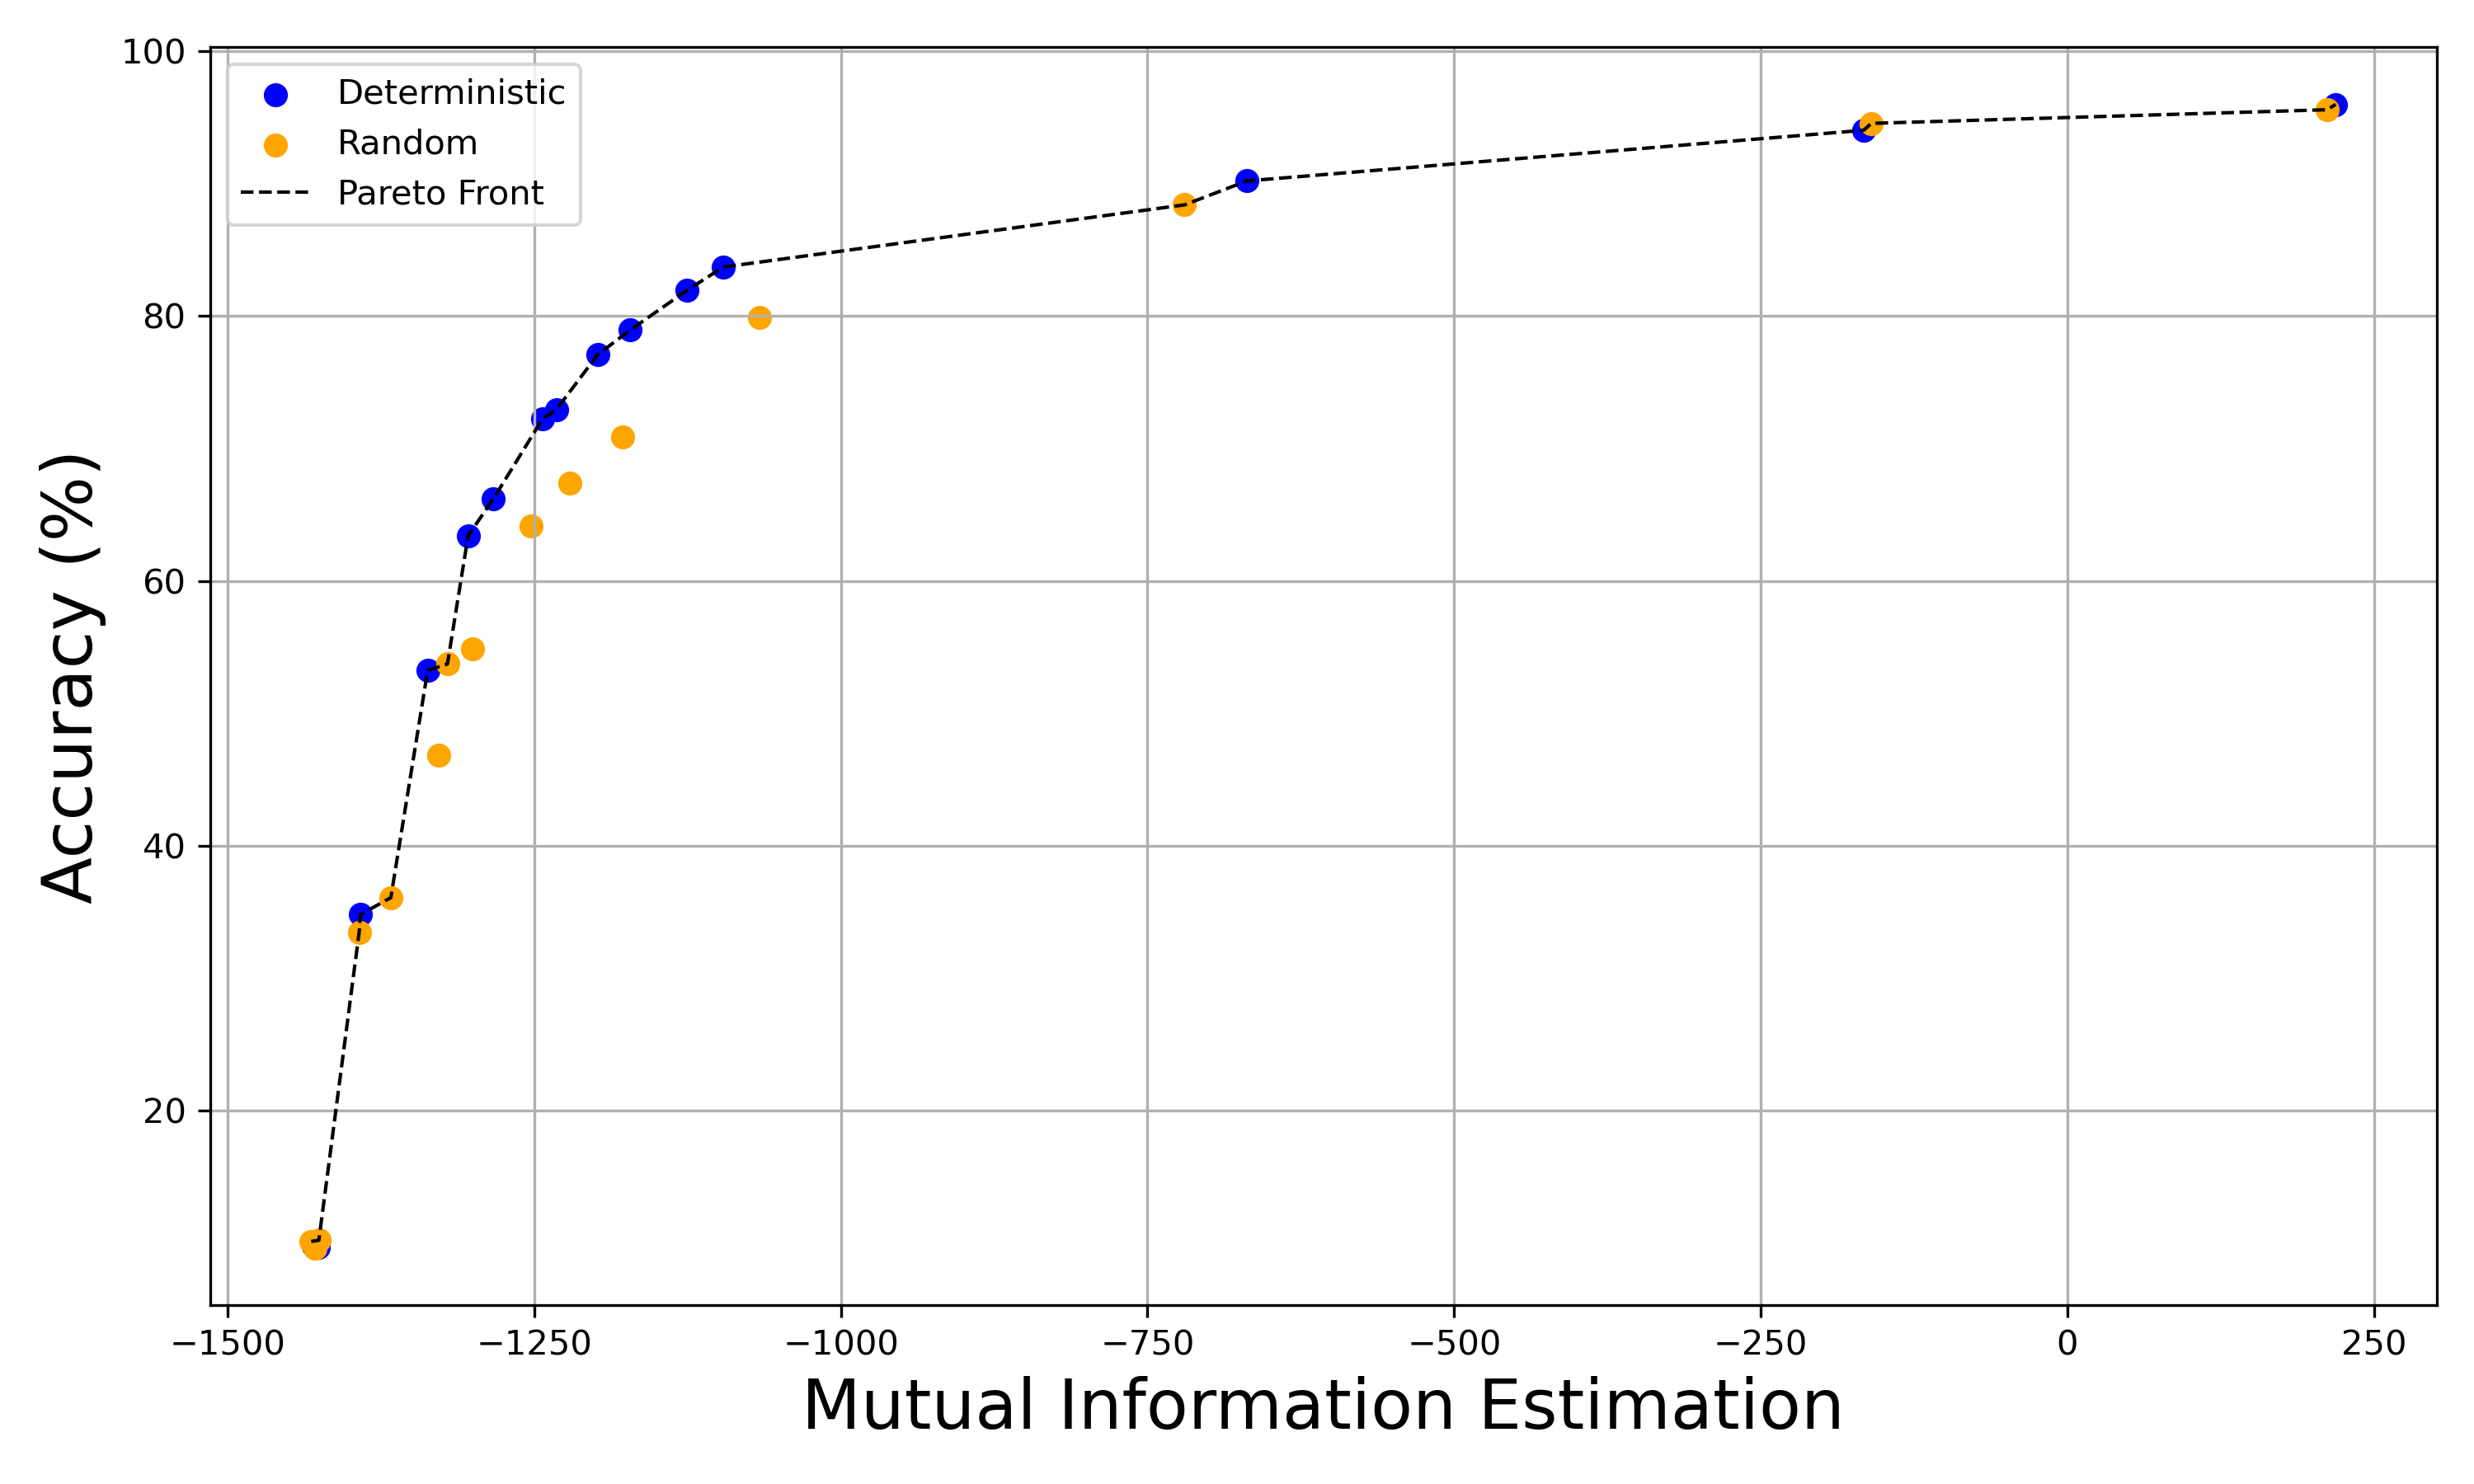
\includegraphics[width=1\textwidth]{conv_pareto_front.png}
            \caption{Models constructed for MNIST.}
            \label{mnist_pareto_front}
        \end{figure}
        We observed that models with deterministic masks consistently outperformed those with random masks along the Pareto front, demonstrating better trade-offs between accuracy and complexity.
        

    The results demonstrate that our method discovers simpler models without compromising predictive accuracy. By incorporating mutual information and complexity regularization, we guide the learning process toward representations that capture relevant patterns in the data. The structure of the learned models reveals the inductive biases inherent in the dataset.  
%------------------------------------------------------------------------------------------------------------
\newpage
\section{Conclusion}
    In this work, we addressed the problem of constructing suboptimal models within the multitask learning paradigm. Given a set of intrinsically related tasks, our objective was to uncover a shared structure---referred to as the inductive bias---common across all tasks. Using constrained evolutionary symbolic regression, we demonstrated that these models could be decomposed in a manner that revealed the underlying structure of the data. We validated our approach through experiments on synthetic data and the MNIST dataset, where the data generation process, structure, and optimal models were known. The results showed that the models produced by the proposed method captured the shared inductive bias, confirming the method's ability to recover interpretable and optimal structures in a multitask setting.
    
    A promising direction is to integrate the proposed method in AutoML pipelines, where the system automatically infers the inductive biases inherent in a given dataset and selects or configures models accordingly. By analyzing symbolic encoders optimized for compression and predictive performance, one could extract structural properties of the data and use these insights to guide model architecture choices.
%------------------------------------------------------------------------------------------------------------
\newpage
% \section{References}    
% \bibliographystyle{plain}
% \bibliography{ib_in_model_selection}
\phantomsection
\addcontentsline{toc}{section}{References}
\urlstyle{rm}
\bibliographystyle{unsrtnat}
\bibliography{ib_in_model_selection}
\urlstyle{tt}

%------------------------------------------------------------------------------------------------------------
\newpage
\section{Appendix}\label{appendix}
    Here we list found models.
    \subsection{Circles}\label{appendix-circles}
    
    \textbf{Model 1:}
    \begin{align*}
    h_0 &= x_0(x_1 + x_1),\\
    h_1 &= (x_0 + p_0) + x_1,\\
    g_0 &= \bigl(p_1 + h_1^2\,p_0^2\bigr) + p_0(p_1 + p_1)(h_0 + h_0),\\
    g_1 &= p_1\,h_0 + p_1 + h_1p_2,\\
    g_2 &= p_2 + (p_1 + h_0)(h_0\,p_0).
    \end{align*}
    
    \textbf{Model 2:}
    \begin{align*}
    h_0 &= (x_0 + p_1)p_0,\\
    h_1 &= \sqrt{x_1^2} + p_2p_0,\\
    g_0 &= \bigl(p_0 + h_0^2\bigr) + \Bigl(p_1^4 + (h_1 + p_0)h_1\Bigr),\\
    g_1 &= h_0^2 + h_1,\\
    g_2 &= p_2h_1 + \sqrt{(h_0 + h_0)^2}.
    \end{align*}
    
    \textbf{Model 3:}
    \begin{align*}
    h_0 &= p_1\bigl(p_2 + p_0 + x_0\bigr),\\
    h_1 &= x_1,\\
    g_0 &= h_1p_0 + \bigl(h_1h_0 + p_2^2\bigr),\\
    g_1 &= h_0^2 + p_0^2 + \bigl(p_1p_2 + p_1\bigr) + p_2h_1^2,\\
    g_2 &= \bigl(p_2 + h_0^2 + \sqrt{h_1^2}\bigr)p_2.
    \end{align*}
    
    \textbf{Model 4:}
    \begin{align*}
    h_0 &= p_2x_0x_1,\\
    h_1 &= x_1 + \bigl(2p_2 + p_0 + x_0 + p_1\bigr),\\
    g_0 &= \bigl(h_0 + p_0 + h_0\bigr)p_0 + h_1^2,\\
    g_1 &= (p_1 + h_0)^4 + p_0p_1h_1,\\
    g_2 &= 2p_1h_1^2 + h_0 + p_2^2.
    \end{align*}
    
    \textbf{Model 5:}
    \begin{align*}
    h_0 &= x_0 + x_1x_0p_1 + x_1 + p_0,\\
    h_1 &= p_2^2,\\
    g_0 &= h_0\bigl(h_0 + p_0\bigr) + \bigl(h_0 + p_0\bigr)^2 + 2h_1,\\
    g_1 &= h_1 + 4p_0^2h_0^2\,p_1^2,\\
    g_2 &= p_1.
    \end{align*}

    \textbf{Model 6:}
    \begin{align*}
    h_0 &= p_1,\\
    h_1 &= x_0^2 + x_1^2,\\
    g_0 &= \bigl(h_0h_1 + 2p_0\bigr)h_1^2 + h_0,\\
    g_1 &= p_0 + \sqrt{h_1} + p_1p_2p_0 + p_0^2p_1 + p_1,\\
    g_2 &= p_0 + \sqrt{h_0^2\sqrt{h_1}}.
    \end{align*}
    
    \textbf{Model 7:}
    \begin{align*}
    h_0 &= \bigl(p_2x_0 + x_1\bigr)^2,\\
    h_1 &= p_1,\\
    g_0 &= h_0 + h_1 + 4h_0^2(h_0 + p_0)^2,\\
    g_1 &= p_2p_1 + \sqrt{h_0}p_1 + p_0,\\
    g_2 &= p_0 + h_0(h_1 + p_2h_0).
    \end{align*}
    
    \textbf{Model 8:}
    \begin{align*}
    h_0 &= x_1^2 + x_0^2,\\
    h_1 &= p_0,\\
    g_0 &= h_1h_0 + p_1\bigl(h_0 + p_1\bigr) + h_0^2p_0^2,\\
    g_1 &= \sqrt{h_0} + h_1,\\
    g_2 &= p_2\bigl(h_0p_0 + p_1 + \sqrt{h_0}\bigr).
    \end{align*}
    
    \textbf{Model 9:}
    \begin{align*}
    h_0 &= p_2,\\
    h_1 &= \bigl(x_1 + x_0p_0\bigr)^2,\\
    g_0 &= \bigl(p_2^2 + p_0\bigr)h_1^2p_2^2 + 2h_1 + p_2,\\
    g_1 &= p_2 + \sqrt{h_1}\bigl(p_2^2 + p_1h_1\bigr),\\
    g_2 &= h_0\sqrt{p_1 + h_1 + h_0^2}.
    \end{align*}
    
    \textbf{Model 10:}
    \begin{align*}
    h_0 &= \bigl(x_1 + x_0\bigr)^2,\\
    h_1 &= p_2,\\
    g_0 &= \bigl(p_1 + h_0\bigr)\bigl(h_1 + p_0 + h_1h_0\bigr) + 2p_1,\\
    g_1 &= \sqrt{h_0}h_1^2 + h_1h_0p_0 + p_1,\\
    g_2 &= h_0p_0 + p_1\bigl(h_1 + p_2\bigr)\sqrt{h_0}.
    \end{align*}
    
    \subsection{4-pixels}
    
    \textbf{Model 1:}
    \begin{align*}
    h_0 &= x_1p_3 -x_2  - p_5 - x_0,\\
    h_1 &= x_2 p_2 + x_3,\\
    g_0 &= \bigl(h_0 + p_1h_0 - h_1h_0 - \max(h_1,p_0)\bigr)\bigl(\max(h_1h_0,p_4 + h_1) + h_0 + p_4p_1\bigr),\\
    g_1 &= h_0\bigl(p_1(p_4 - h_1) - \max(p_3,h_0)\bigr).
    \end{align*}
    
    \textbf{Model 2:}
    \begin{align*}
    h_0 &= x_1,\\
    h_1 &= \max\bigl(p_4,x_2 - x_0\bigr) + x_2p_5 - x_3,\\
    g_0 &= \max\bigl(h_1,\max(p_5,h_1)\bigr) - \max\bigl(p_3, h_1 p_0\bigr) - h_0 p_2(h_1 - h_0),\\
    g_1 &= \max\bigl(h_1 - p_5 - p_0,p_1\bigr) + p_1 + 2p_3h_0(p_3 + h_1)(p_0 + p_5).
    \end{align*}
    
    \textbf{Model 3:}
    \begin{align*}
    h_0 &= \bigl(x_1 + p_2\bigr)\bigl(p_3x_3 + p_1x_2\bigr),\\
    h_1 &= x_1 + p_1x_0,\\
    g_0 &= \max\bigl(h_1 + p_0 - p_5h_0, p_5 - p_4\bigr),\\
    g_1 &= -p_4 + p_5 - \max(h_1,h_1) - (h_0 + p_2) + p_0.
    \end{align*}
    
    \textbf{Model 4:}
    \begin{align*}
    h_0 &= x_1p_3 - x_3\bigl(p_0 + x_2\bigr),\\
    h_1 &= x_0 + x_2p_2,\\
    g_0 &= h_0(h_0 + h_1) + (h_0 + p_4) - p_1p_5\max(h_1,h_1),\\
    g_1 &= (p_1p_2 + p_4 + h_0 + h_1)\max\bigl(p_1p_4, \max(h_1h_0,p_4h_0)\bigr).
    \end{align*}
    
    \textbf{Model 5:}
    \begin{align*}
    h_0 &= p_3\bigl(x_2 - p_4\bigr)\bigl(p_2 + x_0 + x_1\bigr),\\
    h_1 &= x_1\bigl(p_1 - x_3\bigr),\\
    g_0 &= (p_5 - h_0)(p_0 + h_1) - p_4,\\
    g_1 &= \max\bigl(h_0 + h_1,h_0\bigr) + \max\bigl(h_1p_5,p_4\bigr) - \bigl(h_1^2 + p_3\bigr).
    \end{align*}
\end{document}